 \begin{refsection}
\chapter{Catalysis of Na$^+$ Permeation in the Bacterial Sodium Channel Na\textsubscript{V}Ab}

The contents of this section were adapted from an article published in the \textit{Proceedings of the National Academy of Sciences of the United States of America}.\par
\bigskip
Reference: Chakrabarti, N., Ing, C., Payandeh, J., Zheng, N., Catterall, W. A., \& Pom\`es, R. (2013). Catalysis of Na$^+$ permeation in the bacterial sodium channel Na\textsubscript{V}Ab. \textit{Proceedings of the National Academy of Sciences of the United States of America}, 110(28), 11331-11336.\par
\bigskip
Contributions: C.I., N.C, and R.P. designed the research. Simulations were performed by N.C. Data analysis was performed by C.I. and R.P. The manuscript was written by R.P. and N.C. Editorial input and guidance was provided by C.I., J.P., N.Z., and W.C.

\newpage

\section{Summary}

The recent determination of a high-resolution three-dimensional structure of voltage-activated sodium channel Na\textsubscript{V}Ab opens the way to elucidating the mechanism of ion conductance and selectivity.  To examine the permeation of Na$^+$ through the selectivity filter of the channel, we performed large-scale molecular dynamics simulations of Na\textsubscript{V}Ab in an explicit, hydrated lipid bilayer at 0 mV in the presence of 150 mM NaCl, for a total simulation time of 23 $\mu s$.  Although the cytoplasmic end of the pore is closed, reversible influx and efflux of Na$^+$ through the selectivity filter occurred spontaneously in the course of simulations, leading to equilibrium movement of Na$^+$ between the extracellular medium and the central cavity of the channel.  The analysis of Na$^+$ dynamics reveals a knock-on mechanism of ion permeation characterized by alternating occupancy of the channel by 2 and 3 Na$^+$ ions, with a computed rate of translocation of $(6 \pm 1)\times10^{6}$ ions s$^{-1}$ that is consistent with expectations from electrophysiological studies.  The binding of Na$^+$ is intimately coupled to the conformational isomerization of the four E177 side chains lining the extracellular end of the selectivity filter.  The reciprocal coordination of variable numbers of Na$^+$ ions and carboxylate groups leads to their condensation into ionic clusters of variable charge and spatial arrangement.  Structural fluctuations of these ionic clusters result in a myriad of ion binding modes and foster a highly-degenerate, liquid-like energy landscape propitious to Na$^+$ diffusion.  By stabilizing multiple ionic occupancy states while helping Na$^+$ ions diffuse within the selectivity filter, the conformational flexibility of E177 side chains underpins the knock-on mechanism of Na$^+$ permeation.

\section{Introduction}

The rapid passage of cations in and out of excitable cells through selective pathways underlies the generation and regulation of electrical signals in all living organisms \cite{Bezanilla:2008ht,Catterall:2000vb,Catterall:2012fh,Hille:2001tw}. The metazoan cell membrane is exposed to a high-Na$^+$, low-K$^+$ concentration on the extracellular (EC) side, and to a low-Na$^+$, high-K$^+$ concentration on the intracellular (IC) side. Selective voltage-gated Na$^+$ and K$^+$-channels control the response of the cell to changes in the membrane potential.  In particular, voltage-gated Na$^+$-channels (Na\textsubscript{V}) are responsible for the initiation and propagation of action potentials in cardiac and skeletal myocytes, neurons, and endocrine cells \cite{Bezanilla:2008ht,Catterall:2000vb,Catterall:2012fh,Hille:2001tw}. Mutations in Na\textsubscript{V} channel genes are responsible for a wide range of debilitating channelopathies including congenital epilepsy, paramyotonia, erythromelalgia, familial hemiplegic migraine, paroxysmal extreme pain disorder, and periodic paralyses  \cite{George:2005fm,Catterall:2010kr}, underlining the importance of deciphering the relationship between the structure and function of Na\textsubscript{V} channels.  Here we use molecular simulations to study the binding and permeation of Na$^+$ in bacterial sodium channel Na\textsubscript{V}Ab.

Although several atomic structures of K$^+$-selective channels have been solved over the past decade \cite{Doyle:1998wq,Jiang:2003vh,Jiang:2003je}, the atomic structure of a Na$^+$-selective channel from the bacterium \textit{Arcobacter butzleri}, Na\textsubscript{V}Ab, was reported relatively recently \cite{Payandeh:2012ib}.  In the pre-open state of Na\textsubscript{V}Ab, the pore is closed at the IC gate, but the selectivity filter (SF) appears to be in its open, functional state.  The molecular structure of the SF of Na\textsubscript{V}Ab (TLESW) differs significantly from that of potassium channels such as KcsA (TVGYG), in that it is both wider and shorter.  In KcsA, channel coordination of permeating cations consists entirely of direct interactions with backbone carbonyl oxygen atoms.  In contrast, in Na\textsubscript{V}Ab, the SF is lined with amino acid side chains from S178 and E177 in addition to backbone carbonyl groups from T175 and L176 (7, 8, 10, 13). Due to the tetrameric domain arrangement of Na\textsubscript{V}Ab, the E177 site forms a ring of four glutamate side chains (EEEE) in the same sequence positions as the characteristic DEKA ring of eukaryotic sodium channels \cite{Heinemann:1992ep,Terlau:1991ud}. The presence of charged and titratable carboxylate groups in the SF of Na\textsubscript{V} channels raises major questions about the catalytic mechanism for ionic permeation and the structural basis for ion selectivity. 

As a first step toward elucidating the structural basis of ionic permeation and selectivity, we examine the movement of Na$^+$ ions in and out of the pore from equilibrium molecular dynamics (MD) simulations of Na\textsubscript{V}Ab in a hydrated lipid bilayer.  Forty-seven time trajectories totaling 23 $\mu s$ were generated at a temperature of 300 K in the presence of 150 mM NaCl to mimic the physiological environment of the periplasm.  We analyzed Na$^+$ diffusion at a potential of 0 mV, similar to the peak of macroscopic Na$^+$ current during an action potential or a voltage clamp experiment in nerve or muscle cells. The analysis of hundreds of spontaneous events of Na$^+$ diffusion through the SF provides detailed insight into a knock-on mechanism of Na$^+$ permeation involving alternating ion-occupancy states and resulting in an estimated translocation rate of $(6 \pm 1)\times10^{6}$ ions s$^{-1}$. \cite{Payandeh:2012ib}

\section{Results and Discussion}

\subsection{Na$^+$ movement}

\begin{figure}[!ptb]
\centering
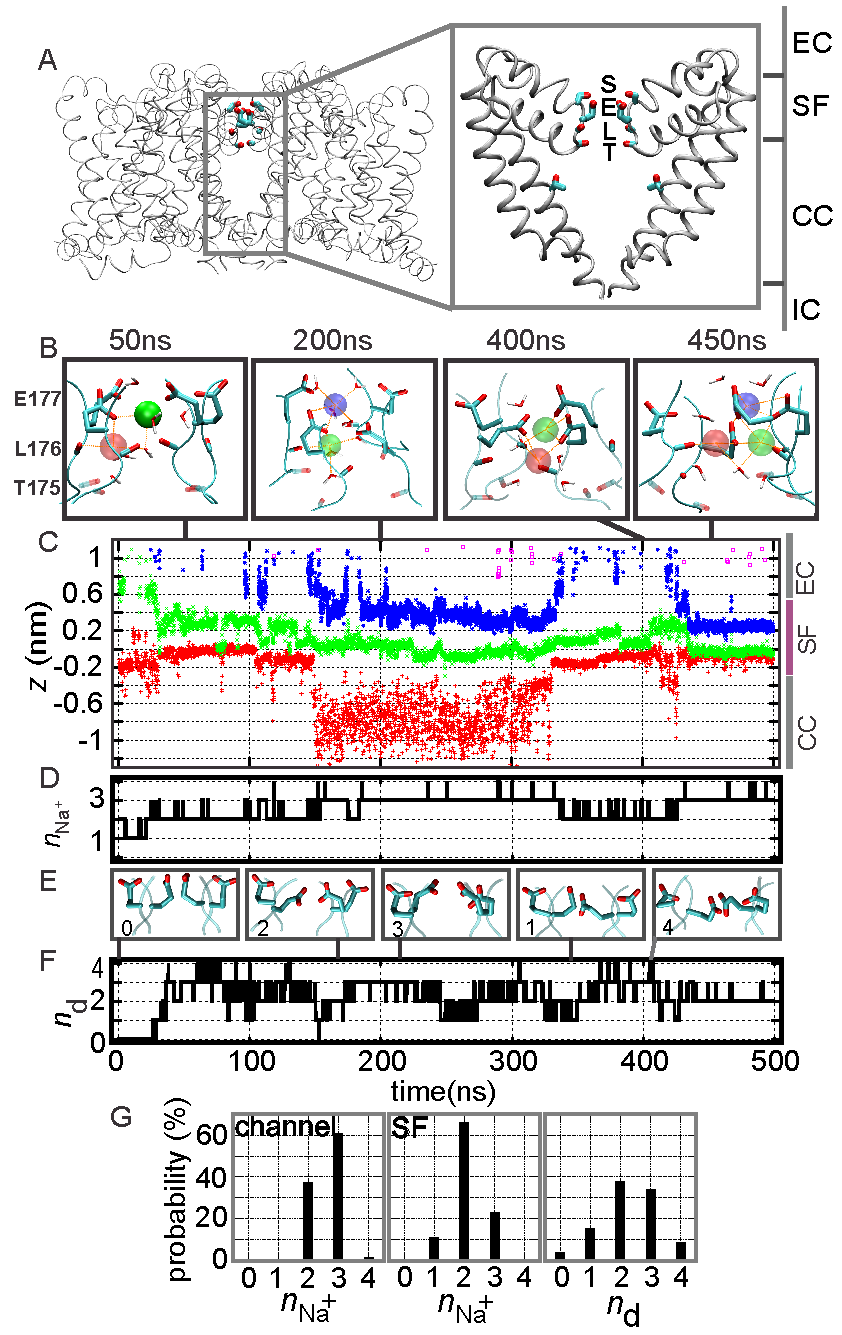
\includegraphics[width=0.5\textwidth]{nav1/Nav1Fig1}
\caption[Sodium movement in the selectivity filter of Na\textsubscript{V}Ab]{\textbf{Sodium movement in the selectivity filter of Na\textsubscript{V}Ab}. (\textbf{A}) Crystallographic structure of Na\textsubscript{V}Ab with a close up of the central ion permeation pore in which the helices above and below the plane of the page have been omitted for clarity.  The constriction of the pore is formed by loops lined with the T175,L176,E177,S178 sequence (the selectivity filter).  The only hydrophilic residue in the central cavity (CC), T206, is also shown.  The IC gate is occluded. (\textbf{B}) Representative snapshots of sodium ions (spheres) in the SF are shown at specified time steps.  The backbone carbonyl groups of T175 and L176 and the side chains of E177 are shown, together with the water molecules involved in the coordination (yellow lines) of permeating ions. (\textbf{C}) Movement of Na$^+$ ions along the pore axis.  By convention, the ions are colored red, green, blue, and purple from the innermost to the outermost position in the channel.  Spontaneous and reversible diffusion of Na$^+$ ions along the channel axis occurred, with visible knock-on and knock-off events at t = 145 and 330 ns, respectively, as the blue and red ions displace each other out of the SF (z = 0 corresponds to the mean axial position of the carbonyl C atom of L176). (\textbf{D}) Time evolution of the number of Na$^+$ ions in the pore. (\textbf{E}) The five conformational states of the EEEE ring, with E177 side-chains pointing either out towards the EC mouth or into the SF lumen (ions not shown). (\textbf{F}) Time evolution of the number of E177 side-chains pointing into the SF. (\textbf{G}) Distribution of ionic populations, and E177 side-chain dunking, from 17 $\mu$s of combined MD trajectories.  Ionic occupancy is shown successively for the entire pore, from the EC funnel to the end of the CC (-0.8 nm $\leq$ z $\leq$ 1.6 nm) and for the SF (-0.53 nm $\leq$ z $\leq$ 0.3 nm).  The pore contains 2, 3 or 4 Na$^+$ ions $36\pm4\%$, $63\pm4\%$, and $2\pm1\%$ of the time, respectively (first panel).  The probabilities of finding 1, 2, or 3 ions in the SF are $11\pm2\%$, $66\pm3\%$, and $23\pm3\%$, respectively (second panel). The probabilities of finding 0, 1, 2, 3 or 4 E177 side-chains in dunked conformations are $4\pm1\%$,$16\pm2\%$, $38\pm3\%$, and $8\pm2\%$, respectively (third panel).}
\label{fig:nav1fig1}
\end{figure}

In the Na\textsubscript{V}Ab structure (Fig. \ref{fig:nav1fig1} A), permeating ions move first into an open extracellular (EC) vestibule, through the narrow SF lined by S178, E177, L176, and T175, and into a central cavity (CC) before exiting through the activation gate.  Although the activation gate at the IC end of the channel is closed, Na$^+$ ions spontaneously traveled in and out of the pore during the course of the simulations (Fig. \ref{fig:nav1fig1} B, C).  The movement of Na$^+$ along the pore axis is shown in two representative 500-ns trajectories and Na$^+$ binding modes (Fig. \ref{fig:nav1fig1} B, C; Fig. \ref{fig:nav1figS2} A,B).  When bound to the channel, Na$^+$ ions were at least partly solvated by one or more carboxylate groups of E177 (Fig. \ref{fig:nav1fig1} B; Fig. \ref{fig:nav1figS2} A).  Using this criterion to define the SF leads to approximate axial SF boundaries of -0.53  z  0.3 nm, where z=0 at the L176 carbonyl.  
In the example depicted in Fig. \ref{fig:nav1fig1}, the first ion (red) permeated through the SF and into the CC, and remained trapped in the pore, occasionally returning to the SF.  A second (green) ion entered the SF at t $\approx$ 21 ns and remained there for the rest of the simulation.  Ionic replacement in the SF occurred at t $\sim$ 150 ns, when the entry of a third (blue) ion forced the expulsion of the red ion to the CC, where it rapidly ``bounced'' up and down as it was no longer directly coordinated to the channel.  This ``knock on'' event was followed by a reverse ``knock off'' process at t $\approx$ 332 ns, when reentry of the red ion into the SF expelled the blue ion to the EC.  Subsequent reentry of a blue ion at t $\approx$ 426 ns did not lead to the expulsion of the red ion from the SF; instead, all three ions resided in the SF for the rest of the trajectory (Fig. \ref{fig:nav1fig1} D).  Na$^+$ movements are accompanied by movements of the side chains of E177 residues, which change their conformation from an outward orientation to an inward ``dunked'' orientation (Fig. \ref{fig:nav1fig1} E-F). 

Although the pore was initially devoid of Na$^+$, two ions penetrated into the channel sequentially within 40 ns in all 47 trajectories.  Based on the time trajectories for a combined 17 $\mu s$ of simulation time, the number of sodium ions present in the pore following this initial equilibration period fluctuated between 2, 3, and 4, respectively 36$\pm$4\%, 63$\pm$4\%, and 2$\pm$1\%  of the time; in the SF, double occupancy (66$\pm$3\%) prevailed over single ($11\pm2\%$) and triple (23$\pm$3\%) occupancy (Fig. \ref{fig:nav1fig1} G).  The average SF occupancy was 2.09 $\pm$ 0.05. Note that the statistical uncertainties reported in this work are the standard error of the mean.

\begin{figure}[!ptb]
\centering
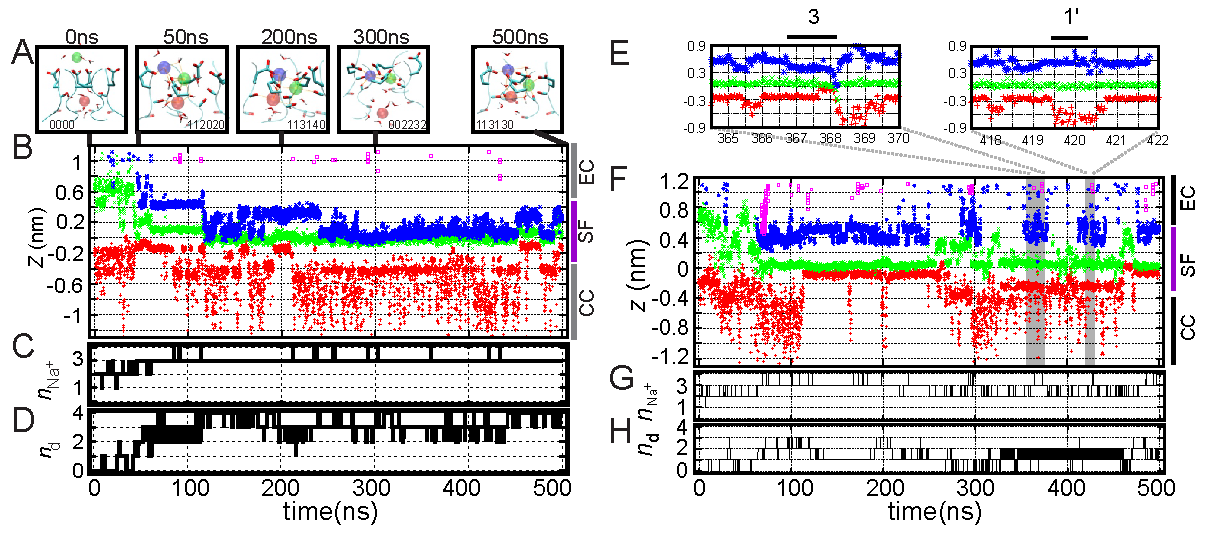
\includegraphics[width=0.9\textwidth]{nav1/Nav1FigS2}
\caption[Two example 500-ns MD trajectories illustrating the dynamics of Na$^+$ ions in the channel lumen]{\textbf{Two example 500-ns MD trajectories illustrating the dynamics of Na$^+$ ions in the channel lumen}. (\textbf{A}) Snapshots of permeating sodium ions, their coordination pattern and the selectivity filter are shown at time steps mentioned.  (\textbf{B,F}) Time evolution of the position of Na$^+$ along the channel axis.  Sodium ions are colored according to their position along channel axis: red, green, blue, and purple, from the innermost to the outermost position, respectively.  In this trajectory, the blue ion remains in the SF following early entry from the EC medium.  (\textbf{C,G}) Number of Na$^+$ ions in the pore. (\textbf{D,H}) Number of E177 side-chains protruding into the lumen (``dunked''). (\textbf{E}) 3-ion and 1- ion intermediate coordination states are highlighted at t = 367-368 ns and t = 420 ns, respectively. }
\label{fig:nav1figS2}
\end{figure}

\subsection{Solvation, Binding, and Energetics of Na$^+$ in the Selectivity Filter}
The movement of Na$^+$ in and out of the pore involves changes in the ionic occupancy of the SF.  To uncover the relationship between ionic binding and mobility, we first decompose the axial distribution of Na$^+$ according to coordination by water and channel groups (Fig. \ref{fig:nav1fig2}).  The axial distribution of channel O atoms in the lumen of the pore is shown in Fig.  \ref{fig:nav1fig2} A.  When in the SF region, Na$^+$ is bound to carboxylate O atoms of E177 only (Fig. \ref{fig:nav1fig2} B, green) or to carboxylates of E177 and carbonyls of L176 together (Fig. \ref{fig:nav1fig2} B, yellow).  Accordingly, we define binding to the SF by carboxylate coordination of Na$^+$.  The bimodal distribution of Na$^+$ in the SF peaks at z = -0.3 and 0 nm, which nearly matches the average positions of E177 carboxyl and L176 carbonyl O atoms, corresponds to two distinct binding modes (E-only and E-, L-bound, respectively). 

\begin{figure}[!htb]
\centering
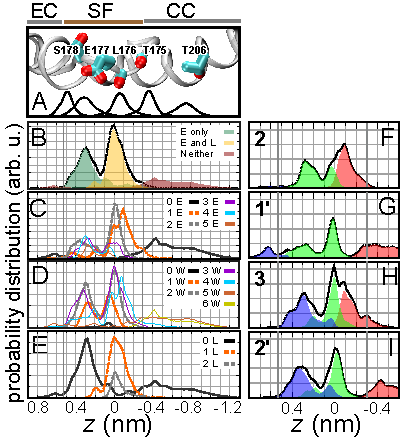
\includegraphics[width=0.5\textwidth]{nav1/Nav1Fig2}
\caption[Sodium binding and occupancy]{\textbf{Sodium binding and occupancy}. (\textbf{A}) Axial distribution of channel O atoms involved in the solvation of permeating Na$^+$ ions, from the hydroxyl groups of S178 and T206, the carboxyl group of E177, and the carbonyl groups of L176 and T175. (\textbf{B}) Axial distribution of Na$^+$ atoms in the SF and CC regions of the channel, distinguishing between states in which Na$^+$ is directly bound to E177 (``E'', green), to both E177 and L176 (``EL'', yellow), or to neither (brown).  The SF is defined by two spatially resolved Na$^+$ binding sites, E and EL.  The small peaks at z = -0.65 and z = 0.40 nm in the brown distribution correspond to direct Na$^+$ coordination by the hydroxyl O atom of S178 and water-mediated coordination to the carbonyl O atom of T175, respectively. (\textbf{C-E}) Decomposition of the axial distribution of Na$^+$ ions according to the number of (\textbf{C}) carboxyl O atoms of E177, (\textbf{D}) water molecules, and (\textbf{E}) carbonyl O atoms of L176 present in the first solvation shell of individual Na$^+$ ions. (\textbf{F-I}) Axial distributions of Na$^+$ ions shown successively for ion coordination macrostates 2, 1', 3, and 2', where integers 1 to 3 correspond to the ionic occupancy of the SF and the prime indicates the presence of one Na$^+$ ion in the CC.  Color coding (red, green, blue) is as defined in the legend of Fig. \ref{fig:nav1fig1}.  The total ionic occupancy of the pore is exactly two in states 1' and 2, and exactly three in states 2' and 3.}
\label{fig:nav1fig2}
\end{figure}

The number of carboxyl O atoms in the first solvation of shell of Na$^+$ varies from 1 to 5 throughout the SF, with 2-4 and 1-2 dominating in the E and EL peaks, respectively (Fig. \ref{fig:nav1fig2} C).  Direct coordination by the channel induces partial dehydration of Na$^+$, with the number of water molecules in the first solvation shell of Na$^+$ dropping from 6 or 7 outside of the SF to a range of 1 to 4 in the SF for nearly all ions (Fig. \ref{fig:nav1fig2} D).  In addition, each Na$^+$ is coordinated by one or occasionally two carbonyl O atoms of L176 in the EL binding site (Fig. \ref{fig:nav1fig2} E).  Variations within the SF reflect the presence of multiple, highly-degenerate ionic binding modes, as discussed below.

The analysis of Na$^+$ coordination leads to four distinct macrostates, which we refer to as 1', 2, 2', and 3.  In this notation, the integer refers to the ionic occupancy of the SF, and primed and unprimed states differ in the number of Na$^+$ present in the central cavity, respectively 1 and 0.  The bimodal character of the axial distribution of Na$^+$ in the SF is retained in all four macrostates (Fig. \ref{fig:nav1fig2} F-I).  The relative population of these two peaks depends on the ionic occupancy of the CC, but not on that of the SF.  When no ion is present in the CC, the relative population of E-only and E-, L-bound peaks is approximately 1:2 (35:65 for state 2 and 33:67 for state 3).  In contrast, when one ion is present in the CC, the two binding sites are nearly equivalent, with E:EL-bound ratios of 45:55 and 50:50 in states 1' and 2', respectively.  This moderate shift in Na$^+$ from the EL site to the E site is likely due in part to repulsive coulombic interactions with the cation in the CC.  

To gain insight into the energetics underlying Na$^+$ movement, we computed two-dimensional free energy surfaces for ion pairs in the channel (Fig. \ref{fig:nav1figS4} A,B).  Analysis reveals a relatively small number of well-defined arrangements of ion pairs in the SF, usually comprised of conformations in which adjacent ions are either distributed in the E-only (z = -0.3 nm) and EL (z = 0) sites, and conformations where two ions are in the EL site, with both cases occurring at once in macrostate 3.  The simultaneous presence of two Na$^+$ ions in the EL binding site is made possible by the relative width of the channel and by coordination of the ions by multiple carboxylate groups.  Rearrangements include either concerted (parallel to the diagonal) or sequential (parallel to one axis) movement of Na$^+$ to and from the above two states, with small intervening barriers (<1 kcal/mol).  These features are relatively independent of ionic occupancy (Fig. \ref{fig:nav1figS4}), revealing the surprising ability of the SF to approximately preserve the energy landscape of Na$^+$ ions. Despite these overall similarities, the free energy landscape governing the movement of Na$^+$ between the SF and the CC depends on both the occupancy and the placement of ions in the SF: when two ions are in the pore, the expulsion of the innermost (red) ion from the SF to the CC requires migration of the second (green) ion from the E site to the EL site (Fig. \ref{fig:nav1figS4} C top). When 3 ions are in the pore, the EL site of the SF is usually occupied by the second ion and there is no longer any barrier impeding movement of the innermost Na$^+$ ion between the SF and the CC (Fig. \ref{fig:nav1figS4} C bottom).  These features support a knock-on mechanism involving either 2 or 3 ions, driven at least in part by coulombic repulsion between Na$^+$ ions.  However, in contrast to the single-file, ``Newton balls'' mechanism of K$^+$ permeation in the narrow SF of K$^+$ channels \cite{MoraisCabral:2001bp}, Na$^+$ conductance in Na\textsubscript{V}Ab does not require concerted cation movement, as two Na$^+$ ions can come side-by-side and occasionally pass each other in the relatively wide SF of Na\textsubscript{V}Ab.

\begin{figure}[hp]
\centering
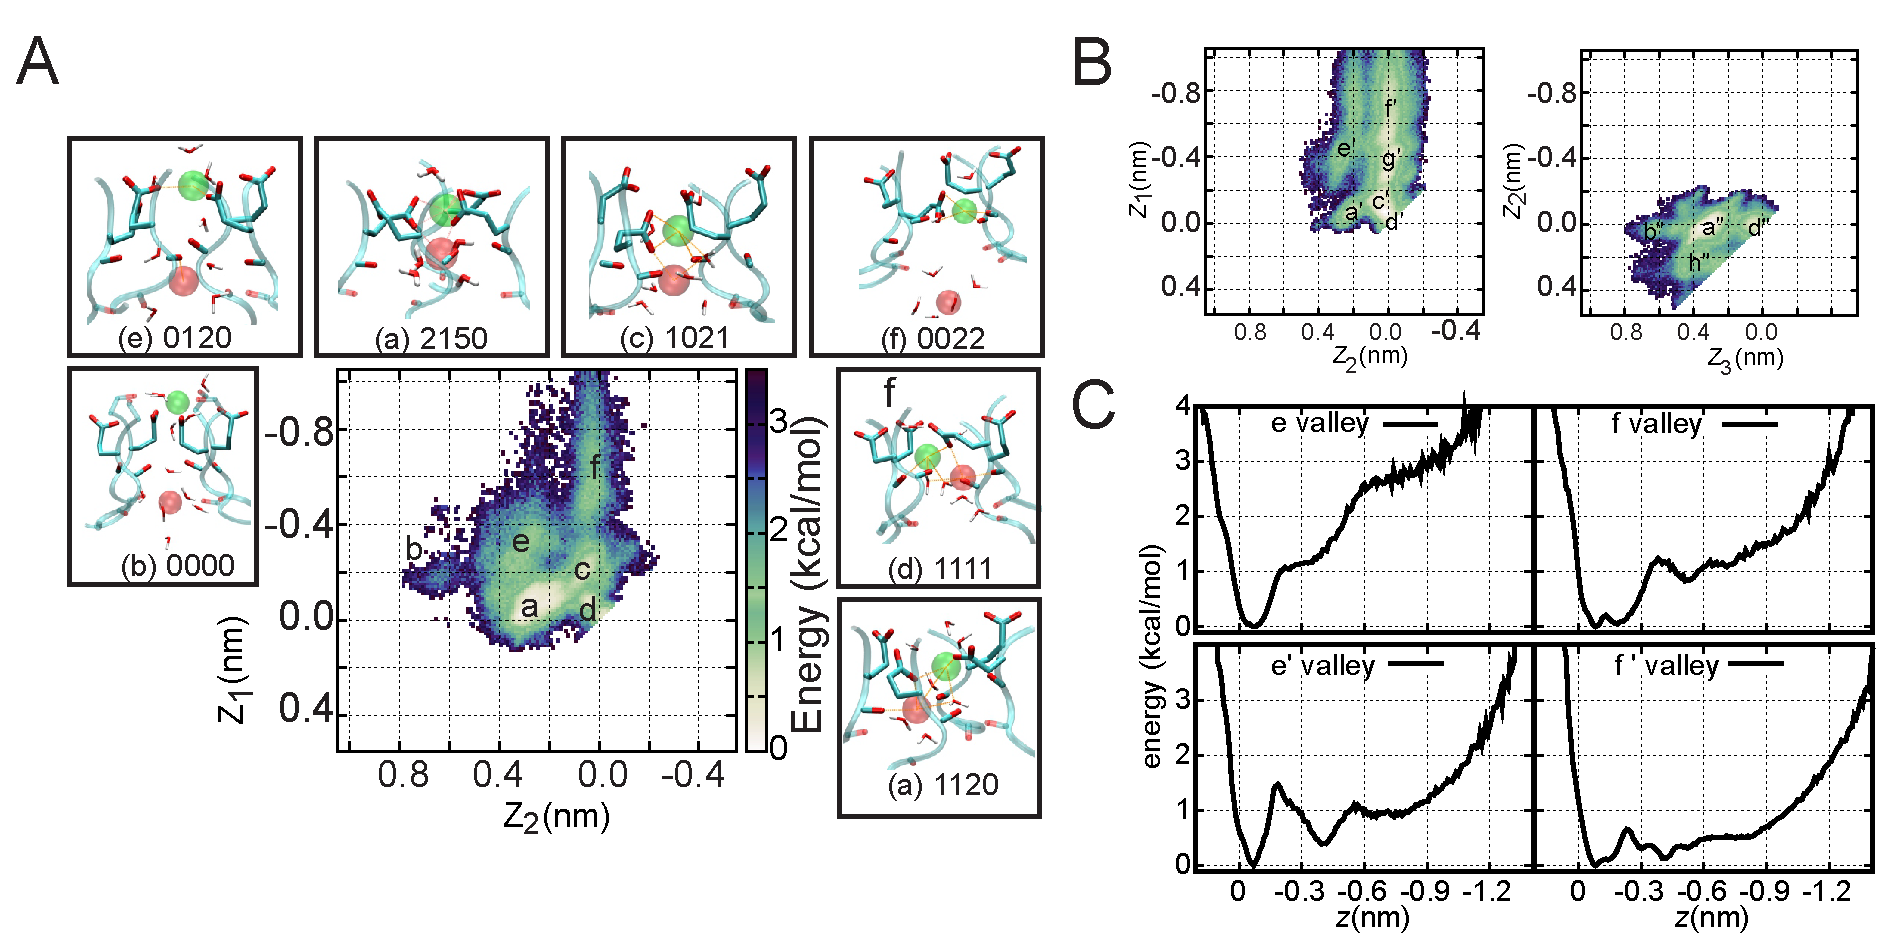
\includegraphics[width=0.9\textwidth]{nav1/Nav1FigS4}
\caption[Free energy landscape of Na$^{+}$ motion in Na\textsubscript{V}Ab]{\textbf{Free energy landscape of Na$^{+}$ motion in Na\textsubscript{V}Ab}. (\textbf{A}) 2D PMF of axial positions of first (red, z$_1$) and second (green, z$_2$) sodium ions in states where two Na$^+$ ions are the channel (macrostates 1' and 2).  The free energy basins are labelled a, c, d, e, and f in order of decreasing occupancy.  Basins a and c are related by concerted ionic motion.  Basin a, the most populated conformation, corresponds to the green and red ions in the E and EL binding modes, respectively (see representative conformations in the insets, where the four-digit code corresponds to E and L coordination).  In basin d, both ions are in the EL-binding mode.   Migration of the green ion from the E binding site (basin e) to the EL binding site (basin f) triggers the expulsion of the red ion into the CC.  (\textbf{B}) 2D PMFs of axial positions of first (red, z$_1$), second (green, z$_2$), and third (blue, z$_3$) sodium ions in triple ionic occupancy macrostates 2' and 3.  (Left) The flat free energy valley defined by d', c', g', and f' suggests that the red ion can diffuse freely between the SF and the CC when the green ion is in the EL binding site (z2 $\approx$ 0).  In basins c' and d', both red and green ions are condensed in the EL binding site.  (Right) Basins b'' to d'' correspond to the stepwise movement of a third (blue) ion in and out of the SF.  Basins a', a'', d', and d'' are equivalent to basins a and d of panel A.  (\textbf{C}) Coupling of ion movement to ionic occupancy of the SF.  Free energy profiles for the movement of the innermost (red) first ion between the selectivity filter (SF) and the central cavity (CC).  The top and bottom panels correspond to total ionic occupancy of two and three Na$^+$ in the channel lumen for (Left) e (top) and e' (bottom) basins; (Right) f and f' basins.  When two ions are in the channel, the expulsion of the innermost ion into the CC is conditional to the presence of a second ion in the EL binding site.  When three ions are in the channel, the presence of the second ion in the EL binding site further facilitates the movement of the innermost ion between the SF and the CC, which becomes diffusive, as suggested by the flat free energy profile in panel f'.}
\label{fig:nav1figS4}
\end{figure}

\subsection{Mechanism and Kinetics of Ion Translocation}

\begin{figure}[!htb]
\centering
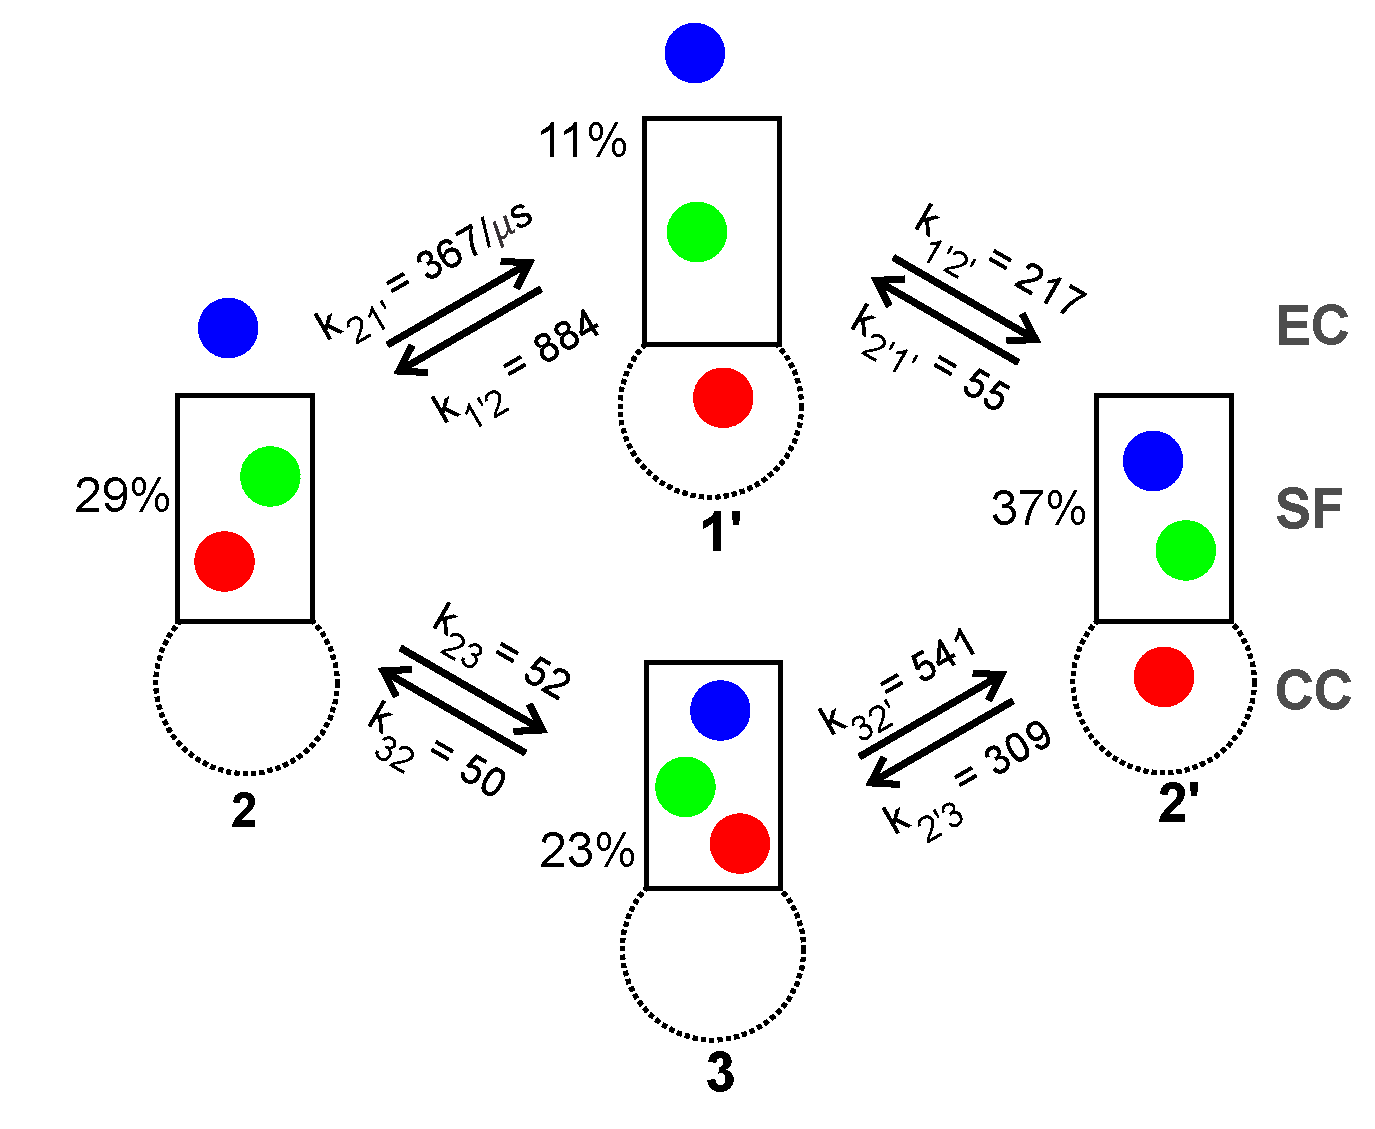
\includegraphics[width=0.9\textwidth]{nav1/Nav1Fig4}
\caption[Mechanism and kinetics of Na$^+$ translocation through the selectivity filter]{\textbf{Mechanism and kinetics of Na$^+$ translocation through the selectivity filter}. The black box represents the SF, with the CC below and the EC mouth above.  Color coding of the ions (spheres) is analogous to that of Figs. \ref{fig:nav1fig1} and \ref{fig:nav1fig2}.  The populations of all four states 1', 2, 2', and 3, which differ in the occupancy of the channel and of the selectivity filter, are shown in \%, and the rate constants computed from the MD trajectories (see Fig. \ref{fig:nav1fig1}) are shown above or below each arrow in units of $\mu s^{-1}$.  At this ionic concentration (150 mM), states 2 and 2' correspond to the resting state of the system. The exchange between states 2 and 2', which corresponds to a unitary ionic translocation through the selectivity filter, involves either one-ion or three-ion intermediate states.}
\label{fig:nav1fig3}
\end{figure}

The analysis of transitions between macrostates 1', 2, 2', and 3 leads to the mechanism depicted in Fig. \ref{fig:nav1fig3} A.  Since two-thirds of all conformations correspond to states 2 and 2', we consider that the resting state of the SF holds two ions, at least in the present, ``pre-open'' state of the channel.  Although a small number of apparently concerted transitions between states 2 and 2' occurred within the time resolution of this analysis (25 ps), most transitions occurred sequentially, either via one-ion or three-ion intermediate states 1' and 3, respectively, depending on whether entry into the SF preceded exit from the SF, or the other way round (a time series illustrating both of these pathways is shown in Fig. \ref{fig:nav1figS2} E-H).  The rates of these transitions are comparable for the two pathways, with the path via the one-ion intermediate being slightly faster.  The mean first passage times for 2$\rightarrow$1'$\rightarrow$2' and 2$\rightarrow$3$\rightarrow$2' translocation events (irrespective of direction) are 0.96 and 6.8 ns, respectively.   

Nearly equal numbers of forward and reverse transitions between the four macrostates depicted were achieved over the set of simulations.  A total of 201 spontaneous Na$^+$ translocation events through the SF occurred within 17 $\mu s$ of simulation, 112 and 75 of which travelled through states 1' and 3, respectively, and 14 of which were direct exchanges.  These ionic permeation events yield an estimated rate of ion flow of $(6 \pm 1 \mu s^{-1}$ through the SF, which is in the range of typical single ion channel permeation rates of 1 to 10 $\mu s^{-1}$ \cite{Hille:2001tw}.  Although the IC gate is closed, this result suggests that the SF is in its functional state and that the rates would not change appreciably if the IC channel gate were open.  The fact that the CC is occupied 48\% of the time indicates that the chemical potential of Na$^+$ in the CC is essentially identical to that in the EC solution at this concentration.  Therefore, the observed diffusion of Na$^+$ through the SF is relevant to Na$^+$ movement in the open state of the channel at 0 mV under conditions of equilibrium (i.e., in the absence of an electrochemical gradient).  

Despite the high mobility of Na$^+$ in the CC (Fig. \ref{fig:nav1fig1} C, Fig. \ref{fig:nav1figS2}), our results suggest that the CC is a binding site for Na$^+$.  The energetics of Na$^+$ binding in the CC and the SF are coupled: there is always one Na$^+$ ion in the CC when a single ion is in the SF (state 1') and triple ionic occupancy of the SF occurs only when the CC is empty (state 3).  However, whether or not the CC is part of the Na$^+$ conduction mechanism may depend on Na$^+$ occupancy at physiological conditions.  Due to the much lower concentration of free Na$^+$ in the cytoplasm (5 mM in humans, 8 mM in \textit{E. coli} \cite{Maguire:2002wu}) than in our simulations (150 mM), the presence of a physiological electrochemical gradient across the membrane is likely to lead to a decreased Na$^+$ occupancy of the CC in the open state of the channel, which could drop by a factor of up to 150/5 = 30.  In that limit, Na$^+$ permeation may occur primarily via alternating macrostates 2 and 3 (Fig. \ref{fig:nav1fig3}), with a higher average occupancy of the SF. 
Regardless of the actual ionic occupancy of the CC, the present study indicates that the permeation mechanism at high Na$^+$ concentration involves the alternation of states in which a total of 2 Na$^+$ (states 2, 1') and 3 Na$^+$ (states 3, 2') are bound in the pore.  The similar population of overall channel occupancy in states 2 and 3 suggests that their exchange underpins an effective knock-on/knock-off process.  Transitions involving the exchange of Na$^+$ between the EC vestibule and the SF are the slowest observed between the four macrostates in Fig. \ref{fig:nav1fig3}, of the order of 50 $\mu s^{-1}$, indicating that the rate-limiting step for the translocation of Na$^+$ through the SF is the migration of the 3rd (blue) ion between the EC and the SF.  By contrast, the movement of Na$^+$ between the SF and the CC is faster by an order of magnitude, a feature that is likely to persist upon directional movement from the SF to the CC in the open state of the channel.

\subsection{Coupling of Channel Structure and Dynamics to Na$^+$ Permeation}

\begin{figure}[!htb]
\centering
\includegraphics[width=0.9\textwidth]{nav1/Nav1FigS8}
\caption[Coupling of channel structure and dynamics to Na+ solvation and mobility]{\textbf{Coupling of channel structure and dynamics to Na+ solvation and mobility}. (\textbf{A}) 2D PMFs of $\chi_{1}$(C$_{\alpha}$-C$_{\beta}$) vs. $\chi_{2}$(C$_{\beta}$-C$_{\gamma}$) for E177 residues successively in the presence (left) and in the absence (right) of excess NaCl salt.  Out-facing and lumen-facing (``dunked'') conformations of E177 are characterized by g$^{+}$ and g$^{-}$ $\chi_{2}$ conformations, respectively.  The presence of Na$^+$ displaces the conformational equilibrium of individual E177 side-chains towards the dunked state. (\textbf{B}) Representative conformations of E177 and S178 side-chains (left) with and (right) without 150-mM NaCl salt; (top) side and (bottom) EC views of the SF.  Conformational dunking allows direct coordination of Na$^+$ ions (left).  In the out-facing conformation, E177 sidechains make hydrogen bonds with the hydroxyl groups of S178 (right). (\textbf{C}) Time evolution of the survival probability of the $\chi_{2}$ dihedral angle of E177 in dunked (``Dunk'') and undunked (``Undunk'') states, shown with a fit to a multiple exponential function.  The fits to the survival probability of the dunked and undunked states in the presence of 150mM NaCl are S(t) = 0.56 exp(-t/0.049)+0.27 exp(-t/0.667)+0.14 exp(-t/8.180) and S(t)=0.51 exp(-t/0.068)+0.29 exp(-t/0.788)+0.16 exp(-t/9.047), respectively, with time t expressed in ns.  In the absence of salt, the exponential fits for dunked and undunked states are S(t) = 0.70 exp(-t/0.012)+0.11 exp(-t/0.09) and S(t)=0.77 exp(-t/0.012)+0.16 exp(-t/0.325)+0.05 exp(-t/8.044), respectively.  Correlation coefficients for these fits were 0.997 or better. (\textbf{D}) Time evolution of the axial projection of centers of cationic charge (CCC) and of anionic charge (CAC) within the channel lumen.  (Black) Average axial position of Na+ ions located inside the SF (0.6$\leq$z$\leq$-0.24 nm, delineated by thick grey lines); (orange) average axial position of carboxylate oxygen atoms of E177 side chains.  Initially, (t$\leq$100 ns), the motions of the CAC and the CCC are uncorrelated (Pearson correlation coefficient p=-0.12), whereas in 100-300 ns and 300-500 ns time segments they show significant correlation (p=0.72 and 0.75).  Based on this analysis, we identify a tight-coupling region (TCR) within which cationic movement is coupled to the movement of E177 side chains.}
\label{fig:nav1figS8}
\end{figure}

Na$^+$ coordination induced rapid and reversible conformational isomerization or ``dunking'' of E177 side chains, bringing their carboxylate group from out-facing to protruding into the lumen (Fig. \ref{fig:nav1fig1} E, F).  Coordination of Na$^+$ by E177 occurred mostly in the dunked conformation, which was much more likely in the presence than in the absence of cations, with the equilibrium constant to dunked vs out-facing conformations of E177 increasing from K$_{dunk}$ = 0.04 $\pm$ 0.02 to 1.7 $\pm$ 0.2 upon addition of salt (Fig. \ref{fig:nav1figS8} A, B).  Moreover, conformational isomerization of E177 occurred on the same time scale as Na$^+$ movement.  Multiple exponential fitting of the survival probabilities of Glu side-chain conformations yields three conformational relaxation times in the order of 0.1, 1, and 10 ns, respectively (Fig. \ref{fig:nav1figS8} A).  The two longer relaxation times are commensurate with the mean first-passage-times of Na$^+$ exchange through the SF, and the longest relaxation time of the dunked state disappears in the absence of salt.  Accordingly, the axial displacement of the center of charge of the carboxylate groups is statistically correlated (Pearson coefficient > 0.7) to that of Na$^+$ ions within the center of the SF region (Fig. \ref{fig:nav1figS8} B).

To uncover the mechanism coupling channel conformational dynamics to ion binding and mobility, we examined the coordination of Na$^+$ by channel O atoms throughout the simulations.  Each microstate (snapshot) was assigned a 6-digit code describing the number of E177 carboxylate and L176 carbonyl O atoms in the first solvation shell of red, green, and blue ions, defining a SF binding mode.  A myriad of distinct ionic coordination states were observed.  A network representation combining the most likely binding modes observed in the entire simulation data set is shown in Fig. \ref{fig:nav1fig5} together with representative snapshots.  Each of these binding modes belongs to one of microstates 1', 2, 2', or 3 and is represented by a node whose area is proportional to its relative population; transitions observed between any two nodes are represented by an edge whose thickness is proportional to flux.  The nodes in the network are highly connected.  This analysis reveals the staggering multiplicity and degeneracy of ionic arrangements combining Na$^+$ ions and COO- groups, whose complementary charges enable their condensation into clusters - particularly in the EL binding site, which often accommodates multiple Na$^+$ ions in close proximity.  In these ionic clusters, Na$^+$ ions are often bound to more than one Glu side chain, and vice versa.  Many individual transitions involve unitary changes in carboxylate O coordination and occur within ~100 ps, the faster timescale of Glu conformational relaxation.  These changes result in the rapid interconversion of ionic arrangements in a fashion reminiscent of a highly-disordered, liquid-like state. 

\begin{figure}[hp]
\centering
\includegraphics[width=0.9\textwidth]{nav1/Nav1FigS7}
\caption[Network representation highlighting the multiplicity and degeneracy of Na$^+$ binding modes]{\textbf{Network representation highlighting the multiplicity and degeneracy of Na$^+$ binding modes}. Each of the four macrostates (1', 2, 2', and 3) corresponds to a large number of microstates (Na$^+$ binding modes) differing in the number of carboxylate O atoms of E177 and carbonyl O atoms of L176 directly coordinating Na$^+$ ions.  Out of a total of 1,233 microstates observed, the 521 most populated binding modes, which account for 99\% of the total population, are depicted as disks whose surface area is proportional to their population.  Each line connecting two states, an edge, represents transitions between these states, with edge thickness proportional to the number of transitions.  The network is clustered and colored using a modularity algorithm which contains no information about the four macrostates, only edge connectivity.  A representative snapshot and the distribution of the number of dunked E177 side-chains are shown as insets for each macrostate.}
\label{fig:nav1fig5}
\end{figure}

More often than not, the ionic clusters are not neutral.  Although there is an overall correlation, there is no simple correspondence between ionic occupancy states and the number of dunked side chains, n$_d$, which fluctuated within all the macrostates (Fig. \ref{fig:nav1fig1} F; Fig. \ref{fig:nav1fig5} insets) and even between closely related microstates.  Charge fluctuations in the ionic cluster result from the impossibility of maximizing attractive interactions between opposite charges while simultaneously minimizing repulsion between like charges and satisfying the spatial constraints imposed by the architecture of the SF.  Together, these factors contribute to the multiplicity and degeneracy of ionic binding modes.  In turn, the fluidity of ionic coordination underpins the high mobility of Na$^+$ in the SF.  By guaranteeing that no single binding mode is significantly stabilized over any other one and that the barriers separating them are low, the conformational flexibility of the EEEE ring shapes an energy landscape conducive to ionic diffusion in the SF and, ultimately, to Na$^+$ permeation. 

\subsection{A Multi-state Knock-on Mechanism for Na$^+$ Permeation in Na\textsubscript{V}Ab}

Our results reveal spontaneous permeation of Na$^+$ through the selectivity filter of Na\textsubscript{V}Ab in a knock-on mechanism involving alternating states in which 2 or 3 Na$^+$ ions are within the pore lumen.  In contrast to the direct solvation of K$^+$ by backbone carbonyl groups in the narrow SF of K$^+$ channels \cite{Doyle:1998wq,Zhou:2001vo}, binding of Na$^+$ in the shorter and wider SF of Na\textsubscript{V}Ab involves both direct and water-mediated interactions of Na$^+$ with the carbonyl groups of T175 and L176 and with the carboxylate groups of E177.  Furthermore, elementary steps of Na$^+$ diffusion in Na\textsubscript{V}Ab do not occur via linear, concerted movement of an ionic column as in the ``Newton balls'' mechanism of K$^+$ permeation in K$^+$ channels \cite{MoraisCabral:2001bp}, but instead involve liquid-like rearrangements of ionic clusters resulting from the condensation of variable numbers of Na$^+$ ions and carboxylate groups.  Evidently, as early in evolution as bacteria, two fundamentally different structures and mechanisms had arisen for conduction of Na$^+$ versus K$^+$ in ion channels.  

In contrast to the classic ``snug'' or ``induced fit'' models of ion permeation, it is becoming recognized that protein flexibility plays a role in selective ion transport \cite{Roux:2011ed,Andersen:2011ty}.  The mechanism uncovered in the present study highlights the interplay of channel dynamics and ion movement.  In the ionic clusters of Na$^+$ and E177 carboxylates in the SF of Na\textsubscript{V}Ab, negative and positive charges are nearly but not exactly compensated.  Far from trapping ions, the reciprocal coordination of permeating Na$^+$ ions and carboxylate groups creates a myriad of ionic binding modes and a highly-degenerate energy landscape propitious to the rapid exchange and diffusion of ions through the SF.  Dynamic coupling of ionic coordination to conformational isomerization of the E177 side chains guarantees at once the multivalency of the SF for Na$^+$ ions and the rapid exchange between alternating states differing in the number of bound ions, resulting in an effective knock-on rate of $6\times10^{6}$ $s^{-1}$.  This unique catalytic mechanism takes advantage of the degeneracy of ionic interactions to accelerate Na$^+$ movement toward the limit of free diffusion.  In upcoming studies, we will examine how this catalytic mechanism is affected by the replacement of Na$^+$ by the other primary physiological cations, K$^+$ and Ca$^2+$, and by the replacement of Glu by the shorter Asp side chain.

In eukaryotes, voltage-gated Na$^+$ channels are composed of four covalently-linked domains similar to one subunit of Na\textsubscript{V}Ab \cite{Hille:2001tw,Catterall:2000vb,Catterall:2012fh,Bezanilla:2008ht}. This arrangement places the amino acid residues DEKA in the positions of EEEE in homotetrameric Na\textsubscript{V}Ab \cite{Heinemann:1992ep}. The mechanism of Na$^+$ permeation described here would be substantially different if DEKA were present at the positions of the four E177 residues in Na\textsubscript{V}Ab.  Further structural and computational studies will be required to understand the mechanistic significance of this profound difference in structure of the SF of bacterial and eukaryotic Na$^+$ channels. 

\section{Methods} 
The simulation system consisted of the Na\textsubscript{V}Ab I217C mutant based on the crystallographic structure with the highest resolution (PDB code: 3RVY) \cite{Payandeh:2012ib}, embedded in a hydrated 1,2-dimyristoyl-sn-glycero-3-phosphatidylcholine (DMPC) bilayer, yielding a system comprising ~219,000 atoms.  The simulations were performed with GROMACS 4.0.7 \cite{Hess:2008db}.  The protein and ions were modeled with the OPLS all-atom force field \cite{Jorgensen:1996vx,Kaminski:2001eq}, and the TIP3P model \cite{Jorgensen:1983ty} was used for water molecules.  The lipid bilayer was modeled by the Berger parameters \cite{Berger:1997bc} using the half-$\epsilon$ double-pairlist method \cite{Chakrabarti:2010gf}.  Forty-seven unconstrained simulations of 400-to-500-ns each yielded 23 $\mu s$ of simulation data.  To check the dependency of our results on the force field, we generated a 340-ns-long simulation with the CHARMM force field \cite{MacKerell:1998tp}. Although this control simulation is too short for a quantitative comparison, results confirm multiple Na$^+$ occupancy in two binding sites involving direct coordination to E177 and L176, as well as conformational isomerization of the Glu side chain and formation of ionic clusters, consistent with the mechanism described above.

\printbibliography[heading=subbibnumbered,title={References}]
 \end{refsection}